\documentclass{standalone}

\usepackage{tikz}

\begin{document}

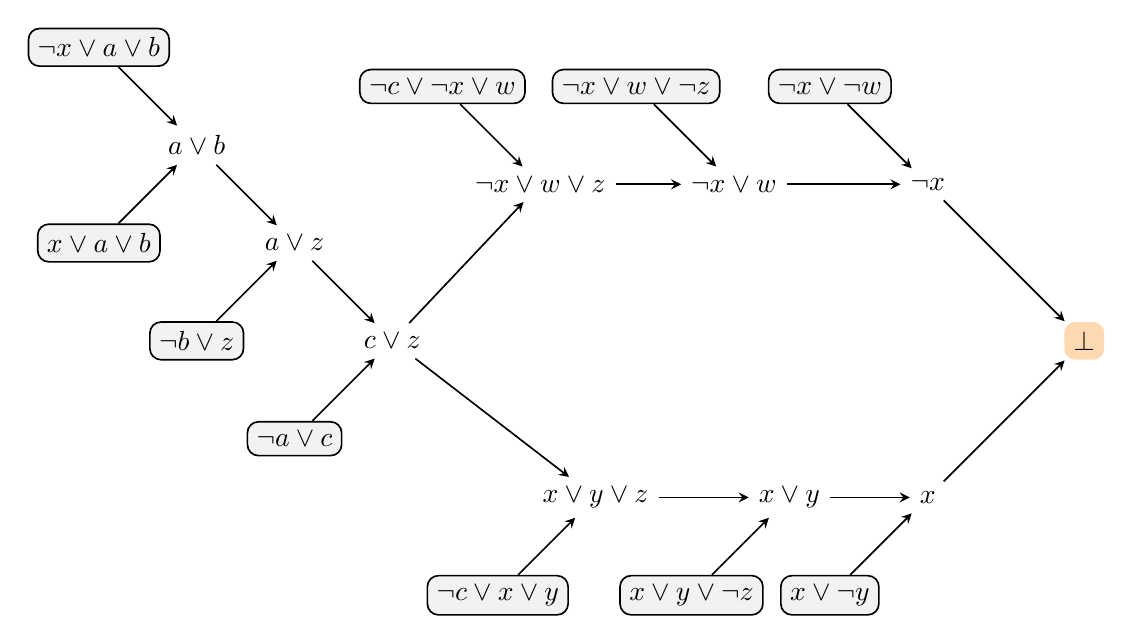
\begin{tikzpicture}

\tikzset{%
every node/.style={fill=white, rounded corners, node distance=5em},%
every path/.style={->, >=stealth, line width=.06em}%
}

\tikzstyle{input}=[draw, fill=black!5!white]
\tikzstyle{bot}=[fill=orange!30!white]


\node[bot] (bot){$\bot$};

\node[below left of=bot, node distance=8em](x){$x$};
\node[above left of=bot, node distance=8em](-x){$\lnot x$};
\draw (x) to (bot);
\draw (-x) to (bot);


\node[input, below left of=x](x-y){$x\lor \lnot y$};
\node[left of=x](xy){$x\lor y$};
\draw (x-y) to (x);
\draw (xy) to (x);

\node[left of=xy, node distance=7em](xyz){$x\lor y\lor z$};
\node[input,below left of=xy](xy-z){$x\lor y\lor \lnot z$};
\draw (xyz) to (xy);
\draw (xy-z) to (xy);

\node[input,below left of=xyz](-cxy){$\lnot c\lor x\lor y$};
\node[left of=bot, node distance=25em](cz){$c\lor  z$};
\draw (-cxy) to (xyz);
\draw (cz) to (xyz);

\node[input,above left of=-x](-x-w){$\lnot x\lor \lnot w$};
\node[left of=-x, node distance=7em](-xw){$\lnot x \lor w$};
\draw (-x-w) to (-x);
\draw (-xw) to (-x);

\node[input,above left of=-xw](-xw-z){$\lnot x\lor w\lor \lnot z$};
\node[left of=-xw, node distance=7em](-xwz){$\lnot x \lor w\lor z$};
\draw (-xwz) to (-xw);
\draw (-xw-z) to (-xw);

\node[input, above left of= -xwz] (-c-xw) {$\lnot c \lor \lnot x \lor w$};
\draw (cz) to (-xwz);
\draw (-c-xw) to (-xwz);

\node[input, below left of=cz](-ac){$\lnot a \lor c$};
\node[above left of= cz] (az){$a\lor z$};
\draw(az) to (cz);
\draw (-ac) to (cz);

\node[input, below left of=az](-bz){$\lnot b \lor z$};
\node[above left of= az] (ab){$a\lor b$};
\draw(-bz) to (az);
\draw (ab) to (az);

\node[input, below left of=ab](xab){$x \lor a \lor b$};
\node[input,above left of= ab] (-xab){$\lnot x \lor a\lor b$};
\draw(xab) to (ab);
\draw (-xab) to (ab);
	
\end{tikzpicture}

	
\end{document}
